%%%%%%%%%%%%%%%%%%%%%%%%%%%%%%%%%%%%%%%%%%%%%%%%%%%%%%%%%%%%%%%%%%%
%                                                                 %
%                            CHAPTER FOUR                         %
%                                                                 %
%%%%%%%%%%%%%%%%%%%%%%%%%%%%%%%%%%%%%%%%%%%%%%%%%%%%%%%%%%%%%%%%%%%

\chapter{RESULTS}\label{ch:implement}

\section{Introduction}

When versioning a data set, researchers very rarely ask whether two objects can be compared.
The data producer often establishes the context in which data objects are sufficiently similar---to use terms from FRBR---\textbf{expressions} of the same \textbf{work}.
Confirming the context prior to making version comparisons is fundamental to ensuring that the resulting versioning graph contains meaningful results.
The data sets described in the following section have sufficient context as established by their producers.
Using the data in these data sets, the model from Chapter \ref{ch:model} is instantiated into versioning graphs.
The graphs are encoded into HTML change logs using RDFa and JSON-LD.
These graphs allow for an analysis of the change between versions, which gives insight into the version identifier.
Finally, a version graph is used to classify the kinds of change separating versions of a data set to determine the utility.

\section{Utilized Data Sets}

\subsection{Noble Gas Data set}

The ``Global Database on \textsuperscript{3}He/\textsuperscript{4}He in on-shore free-circulated subsurface fluids" is a tumultuous database \cite{Polyak2015}.
The first version, published in June 11, 2013, contains 8 files with 194 columns each.
The next version of the database, published March 8, 2015, compiles all the data into a single file and reduces the number of columns to 54, marking a drastic change.
In addition, several columns changed the units with which they reported measurements.
While usage documentation, explaining the content and use of the data, accompanied each version, no records were included indicating what changed between versions.
A change log would be valuable guide with such drastic structural and content changes.
The third and most recent publication came in July 11, 2017, with no changes to the number of files or columns, but many new rows.

\subsection{Copper Data set}

The Paragenetic Mode for Copper Minerals database became available through collaboration with the author's lab to create new methods of visualizing mineralogy relationships \cite{Morrison2016}.
The first version was collected June 8, 2016, with the update following soon after on August 8, 2016.
Major edits are fairly limited with only 16 column additions and 2 removals between the versions.
Value formats remain consistent from one version to the next, resulting in a much more condensed body of changes, making transitions more easily verifiable.
Compared to the Noble Gas data set, it provides a more stable data platform to implement the versioning model in Chapter \ref{ch:model}.
The data from this work is also more processing friendly, making it agreeable to automatic change log generation.

\subsection{GCMD Keywords}

The Global Change Master Directory (GCMD) is a metadata repository used by NASA to store records of its available data sets \cite{Miled:2001:GCM:372202.372324}.
They employ a set of keywords to make NASA Earth Science data sets searchable.
These words tag and label datasets into strictly defined categories \cite{GCMDKey}.
GCMD Keywords do not qualify as a standard web ontology since it does not constitute a class hierarchy.
The management team stored early versions of the keywords in Excel spreadsheets, and a centralized distribution system was not used until June 12, 2012.
The Key Management Service now serves the keywords directly in a variety of formats.
Each version of the keywords, encoded in RDF, were downloaded into separate files.
Only versions from June 12, 2012 and after were available, resulting in 9 version files.
Each keyword corresponds to a unique identifier, and when combined with a web namespace, resolves to a data description of the keyword.
Every identifier can be referred to per version by including the version's number at the web identifier's end, meaning that identifiers are consistent across versions.
The taxonomy uses the concepts \textit{skos:Broader} and \textit{skos:Narrower}, where skos refers to the Simple Knowledge Organization System ontology name space, to form a tree hierarchy \cite{skos}.
The tree's root is the keyword, "Science Keywords."
The data set provides an interesting study case due its long sequence of versions and ready use of linked data technology \cite{Stevens2016}.

\begin{table}
	\caption{List of versions available in the KMS.}
	\label{gcmd_table}
	\centering
	\begin{tabular}{|c|c|c|c|c|c|c|c|c|}
		\hline
		June 12, 2012 & 7.0 & 8.0 & 8.1 & 8.2 & 8.3 & 8.4 & 8.4.1 & 8.5 \\
		\hline
	\end{tabular}
\end{table}

\subsection{MBVL Classifications} \label{sec:MBVL}

The Marine Biodiversity Virtual Laboratory (MBVL), based at Woods Hole Oceanographic Institution, provides data and services for the study of marine biology with an integrative approach \cite{mbvl}.
In the application studied, a choice of algorithm and taxonomy pairings must be tested on a known population in order to estimate their performance with an unknown microbial population.
The original sequences belong only to the species listed in Table \ref{species_table}.
The original population's census is not available to the author, and only the list of species are known, forming the first data set in this section.
These sequences are then grouped and classified by a specific taxonomy and algorithm pairing.
The workflow utilizes two taxonomies, the Ribosomal Database Project (RDP) and the Silva taxonomy.
Using these databases, the Species-level IdentificatioN of metaGenOmic amplicons (SPINGO) or the Global Alignment for Sequence Taxonomy (GAST) algorithms assign taxonomic ranks to each sequence.
The process produces four data sets, each using the same grouping identifiers and having the same size in each group.
Since the data sets have the same number of sequences, the primary difference between the data sets are the ranks assigned to each sequence.

\begin{table}
	\caption{List of species in the original population.}
	\label{species_table}
	\centering
	\setlength{\tabcolsep}{2pt}
	\begin{tabular}{|c|c|c|}
		\hline
		Acinetobacter baumannii & Actinomyces odontolyticus & Bacillus cereus \\
		Bacteroides vulgatus & Clostridium beijerinckii & Deinococcus radiodurans \\
		Enterococcus faecalis & Escherichia coli & Helicobacter pylori \\
		Lactobacillus gasseri & Listeria monocytogenes & Neisseria meningitidis\\
		Porphyromonas gingivalis & Propionibacterium acnes & Pseudomonas aeruginosa \\
		Rhodobacter sphaeroides & Staphylococcus aureus & Staphylococcus epidermidis\\
		Streptococcus agalactiae & Streptococcus mutans & Streptococcus pneumoniae \\
		\hline
	\end{tabular}
\end{table}

\section{Implementing the Versioning Model}

The following subsections detail the steps used to implement a versioning graph using the model defined in Chapter \ref{ch:model} and the challenges encountered.
Section \ref{mapping} goes through the decisions made to align the attributes within the Noble Gas dataset and within the Copper data set.
The alignments create a formula to detect changes and assign them to either an \textbf{add}, \textbf{invalidate}, or \textbf{modify} change.
A change log can then use the assignments to organize a presentation of the change data.
The underlying versioning graph exists as linked data encoded within the change log, but can also appear as explicit linked data statements.
The procedure within this section defines the process used to create versioning graphs found in all the following sections of this chapter.

\subsection{Form a Mapping} \label{mapping}

A mapping specifies the method to determine the \textbf{attributes} of a versioning graph and how to compare them.
For spreadsheets and table-based data, row and column indexes initially seem an ideal attribute, but edits often show the contrary.
The Noble Gas data set needed a mapping to align the spreadsheet's columns since 140 columns were removed from the first version.
The remaining columns in the second version no longer had the same column indexes that they did in version 1 so the column headers were used instead.
The Copper data set retains many of the original columns, but their ordering has changed between versions.
In addition, rows must be aligned since both a row and column attribute are necessary to uniquely identify a cell.
Cells need to be uniquely identified since this is where a comparison will be made to determine whether a \textbf{modify} change has occurred in a spreadsheet.

Once aligned, determining which attributes have been added, invalidated, or modified is straight-forward.
Attributes which only exist in the original or left-hand version have been invalidated.
More specifically, a set of attributes \(\mathcal{I} = \mathcal{R}_{l} - \mathcal{R}_{r}\) where \(\mathcal{R}_{l}\) and \(\mathcal{R}_{r}\) correspond to the row identifiers of the left-hand and right-hand versions, respectively.
Likewise, a set of attributes \(\mathcal{A} = \mathcal{R}_{r} - \mathcal{R}_{l}\) contain all the added attributes.
Performing the same operations on the columns result in sets of the added and invalidated columns.
A script then iterates over the remaining cells which exist in both versions to determine if they differ, resulting in a \textbf{modify} change.
The unchanged cells form a set of entries which do not appear in a change log or the versioning graph.
The attributes in these sets are then minted into URIs and linked together into the versioning graph, or they can be used to publish a change log.

\subsection{Produce Change Log}

Change logs were generated for both the Noble Gas data set and the Copper data set.
Following the practices of other change logs, the documents present before and after values for comparison which can be seen in Figure \ref{changelog_zoomed}.
\begin{figure}
	\centering
	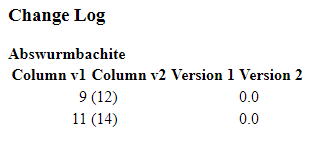
\includegraphics[scale=0.80]{figures/Changelog-zoomed.png}
	\caption{Abswurmbachite entry in the Copper Dataset Change Log}
	\label{changelog_zoomed}
\end{figure}
The partial snapshot of the change log shows that column numbers in the Copper data set also accompany the values to identify the data's location in the spreadsheet.
Very little natural language is used in this change log to regularize the format and improve compatibility with RDFa.
The change logs follow a common format with three sections: Additions, Invalidations, and then Modifications.
The sections may be further grouped by column or row additions.
The division means that changes are not published into the change log as they are found, but instead organized and grouped beforehand.

Employing RDFa means that the document must be written using HTML formatting.
Listing \ref{rdfa_list} shows the text necessary to layout the first four lines of Figure \ref{changelog_zoomed}.
While the content only shows four lines, the underlying markup takes up three and a half times as many lines.
Line 2 states that all following resources will be \textbf{attributes} of Version 1.
Line 3 defines such an \textbf{attribute}.
Lines 5 through 8 define the changes Abswurmbachite undergoes.
Because RDFa allows the statements to be embedded within the content, the triples can appear along with the text they describe.
Lines 11 and 12 define complete triples which do not appear in the visible document.
The lines complete the graph, but must be included in spans because RDFa only allows a single triple within each tag.
Modifying the tags' order so that the spans are unnecessary would cause the visible content to appear in an un-logical order, rendering the document machine-readable but not human-readable.

\begin{lstlisting}[language=HTML, caption=Abswurmbachite RDFa, label=rdfa_list]
<h3>Change Log</h3>
<div about="Version1" rel="vo:hasAttribute">
  <div resource="v2:Abswurmbachite" typeof="vo:Attribute">
    <span style="font-weight:bold" property="http://www.w3.org/2000/01/rdf-schema#label">Abswurmbachite</span>
    <table rel="vo:Undergoes">
      <tr  about="ChangeAbswurmbachite12" typeof="vo:Change">
        <td align="right" rev="vo:Undergoes" resource="v1:AttributeAbswurmbachite12v1" typeof="vo:Attribute"> 9</td>
        <td property="vo:resultsIn" resource="v2:AttributeAbswurmbachite12v2" typeof="vo:Attribute">(12)</td>
        <td>          </td>
        <td>       0.0</td>
        <span about="Version1" property="vo:hasAttribute" resource="v1:AttributeAbswurmbachite12v1"></span>
        <span about="Version2" property="vo:hasAttribute" resource="v2:AttributeAbswurmbachite12v2"></span>
      </tr>
    </table></div></div><br>
\end{lstlisting}

After encountering the limitations of using RDFa to include the versioning graph into the change log, JSON-LD was used.
The new format does not rely on the structure of visible content to determine the syntax triples use to be included in the change log.
Listing \ref{json_list} provides the alternative encoding of the Abswurmbachite entry from RDFa.
The entry is significantly longer, almost three times longer than the RDFa entry and ten times longer than the original visible content.
Instead of including all the data in the beginning or end of the document, each change block is separated into the particular \textit{div} section for that change.
This choice allows consumers to extract pertinent change information without needing to ingest the entire versioning graph.

\begin{lstlisting}[language=HTML, caption=Abswurmbachite JSON-LD, label=json_list]
<h3>Change Log</h3>
<div about="v1:Abswurmbachite">
  <span style="font-weight:bold" property="http://www.w3.org/2000/01/rdf-schema#label">Abswurmbachite</span>
  <table>
    <tr  id="ModifyChangeAbswurmbachite12">
      <td align="right"> 9</td>
      <td >(12)</td>
      <td>          </td>
      <td>       0.0</td>
      <script type="application/ld+json">
[
{
	"@context": "https://orion.tw.rpi.edu/~blee/provdist/GCMD/VO.jsonld", 
	"@id": "http://CUdb.com/v1/AttributeAbswurmbachite9", 
	"@reverse": {
		"hasAttribute": "Version1"
	}, 
	"@type": "vo:Attribute", 
	"label": "Primary", 
	"undergoes": "http://orion.tw.rpi.edu/~blee/provdist/CU/DTDI/CUjsonlog.html#ModifyChangeAbswurmbachite12"
}, 
{
	"@context": "https://orion.tw.rpi.edu/~blee/provdist/GCMD/VO.jsonld", 
	"@id": "http://orion.tw.rpi.edu/~blee/provdist/CU/DTDI/CUjsonlog.html#ModifyChangeAbswurmbachite12", 
	"@type": "vo:ModifyChange", 
	"resultsIn": "http://CUdb.com/v2/AttributeAbswurmbachite12"
}, 
{
	"@context": "https://orion.tw.rpi.edu/~blee/provdist/GCMD/VO.jsonld", 
	"@id": "http://CUdb.com/v2/AttributeAbswurmbachite12", 
	"@reverse": {
		"hasAttribute": "Version2"
	}, 
	"@type": "vo:Attribute", 
	"label": "Primary"
}
]
      </script>
    </tr>
  </table></div><br>
\end{lstlisting}

The encoded change logs struggle with intense document size.
The Copper Minerals data set encoded in RDFa is 1.7 MB and JSON-LD is 3.3 MB.
In the Noble Gas data set, the RDFa and JSON-LD change log sizes are 59 and 60 MB, respectively.
The Noble Gas change logs often do not load in a browser.

\begin{table}[b]
	\caption{Sizes of change log encodings.}
	\label{changelog_table}
	\centering
	\begin{tabular}{|c|c|c|c|}
		\hline
		Dataset & No Encoding & RDFa (MB) & JSON-LD (MB) \\
		\hline
		Copper Minerals &  & 1.7 & 3.3 \\
		Noble Gas &  & 59 & 60 \\
		\hline
	\end{tabular}
\end{table}

\subsection{Generate Versioning Graph}

The versioning graphs presented in this section were created by extracting triples from the associated change log.
The statements making up the graph could have alternately been published by writing out the triples directly instead of encoding them into a change log.
Figure \ref{NobleGraph1} displays a subgraph of the Noble Gas data set's versioning graph between versions 1 and 2, highlighting each of the three change operations.
\begin{figure}
	\centering
	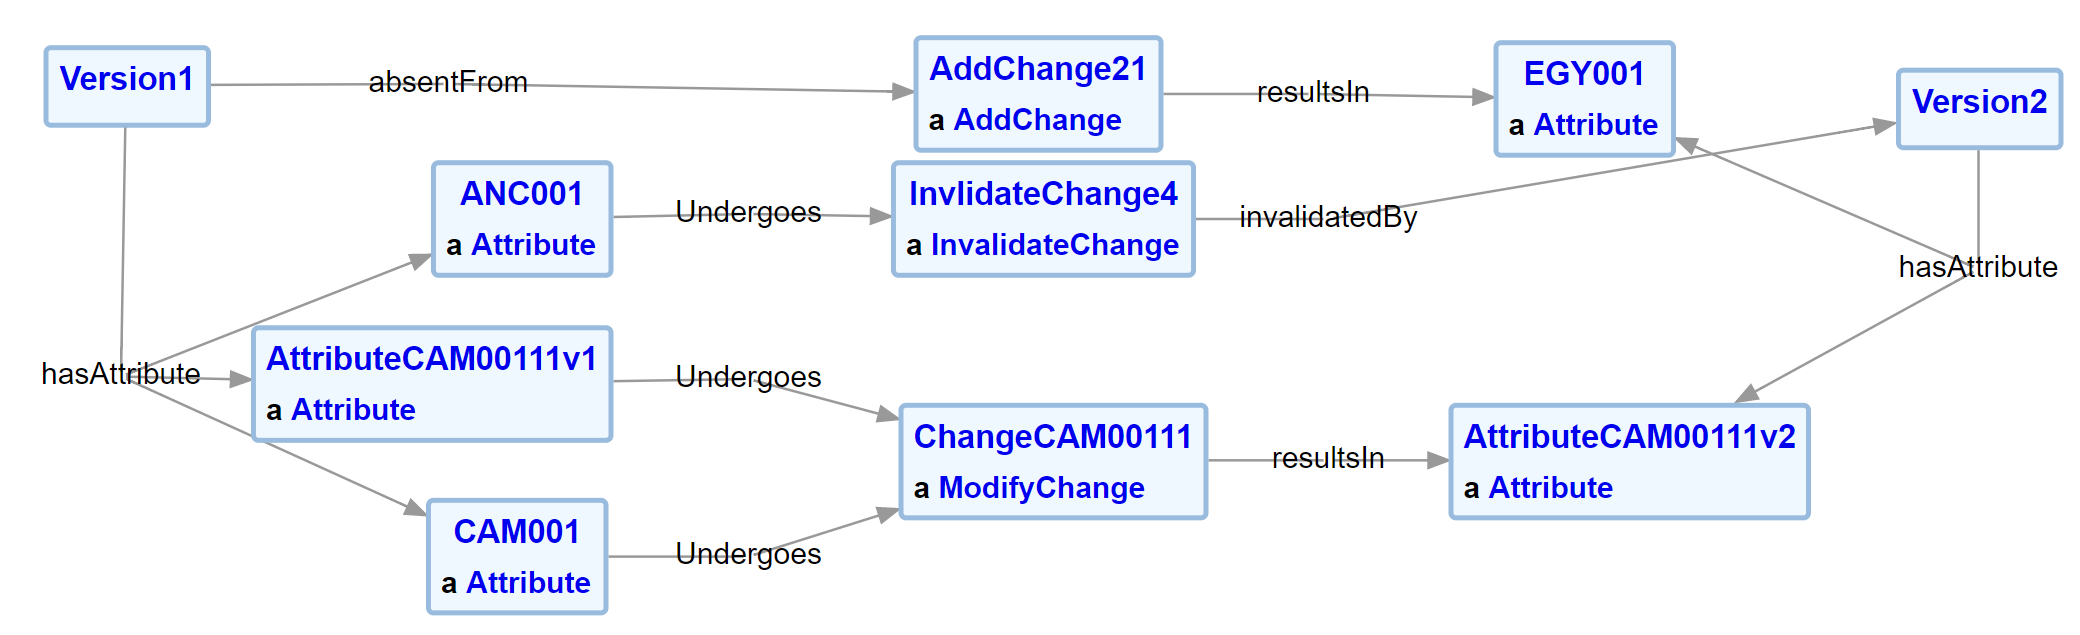
\includegraphics[scale=0.30]{figures/NobleVersion.png}
	\caption{Some initial entries from versions 1 and 2 of the Noble Gas data set}
	\label{NobleGraph1}
\end{figure}
Notice how the versioning graph differs from the provenance graph in Figure \ref{CAM001ProvGraph}.
The versioning graph unpacks the \textit{prov:wasRevisionOf} relationship into explicit components.
These components reveal more detailed differences between version 1 and 2 of CAM001 in the provenance graph which are the differing compilation activities.
\begin{figure}[b]
	\centering
	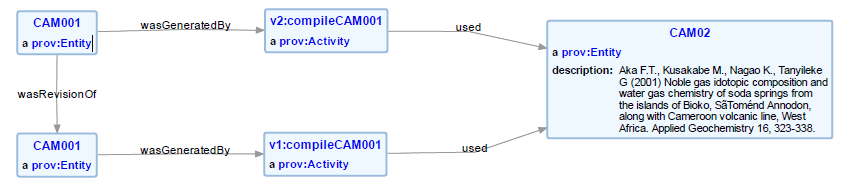
\includegraphics[scale=0.70]{figures/CAM001v1v2.png}
	\caption{Provenance graph for the CAM001 entry of the Noble Gas Database.  Other than the labels, the structure of each data object is very much the same.}
	\label{CAM001ProvGraph}
\end{figure}
The change log encoded the triples in RDFa, resulting in the attribute ``AttributeCAM00111v2" to the right of the \textbf{modify} change.
Because RDFa does not naturally support multiple predicates while also conforming to the content structure of the change log, an attribute was created to combine both the row and column identifier for the changing cell.
Separating the attributes would require multiple dedicated HTML tags which don't appear along with content.
Including these tags would diverge from benefits of encoding triples as attributes.
Figure \ref{NobleGraph1} also shows that even though many columns are added when a new row is added, the row identifier can be used to summarize the columns additions.

Listing \ref{NGA} presents the statements in turtle format necessary to express that the entry EGY001 has been added to the data set from Version 1 to Version 2 as shown along the top of Figure \ref{NobleGraph1}.
The namespace for many of the URIs is \textlangle http://rdfa.info/play/\textrangle.
RDFa allows identifiers to refer to an element on the web page, and the web tool which generated the triples from RDFa, therefore, used its URL as a namespace to produce a valid URI.

\begin{lstlisting}[language=SPARQL, caption=Noble Gas Add in Turtle, label=NGA]
<http://rdfa.info/play/Version1> a vo:Version ;
vo:absentFrom <http://rdfa.info/play/AddChange21> .
<http://rdfa.info/play/AddChange21> a <https://orion.tw.rpi.edu/~blee/VersionOntology.owl#AddChange> ;
vo:resultsIn <http://rdfa.info/play/Attribute21> .
<http://rdfa.info/play/Attribute21> a <https://orion.tw.rpi.edu/~blee/VersionOntology.owl#Attribute> ;
rdfs:label "EGY001"
<http://rdfa.info/play/Version2> a vo:Version ;
vo:hasAttribute <http://rdfa.info/play/Attribute21>
\end{lstlisting}

Figure \ref{CopperGraphVerGraph} shows a similar subgraph from the Copper data set versioning graph.
The graph was assembled using an RDFa change log and also displays a merged attribute on the right side of the \textbf{modify} change.
In the full versioning graph, multiple of each change is present, forming a zipper or ladder-like structure.
As a result, each \textbf{add}, \textbf{invalidate}, or \textbf{modify} change is given separate names for each instantiation.

\begin{figure}
	\centering
	\begin{adjustbox}{addcode={\begin{minipage}{\width}}{
					\caption{Versioning Graph representing the linked data graph with selected entries of additions, invalidations, and modifications. 
			}\end{minipage}},rotate=90,center}
		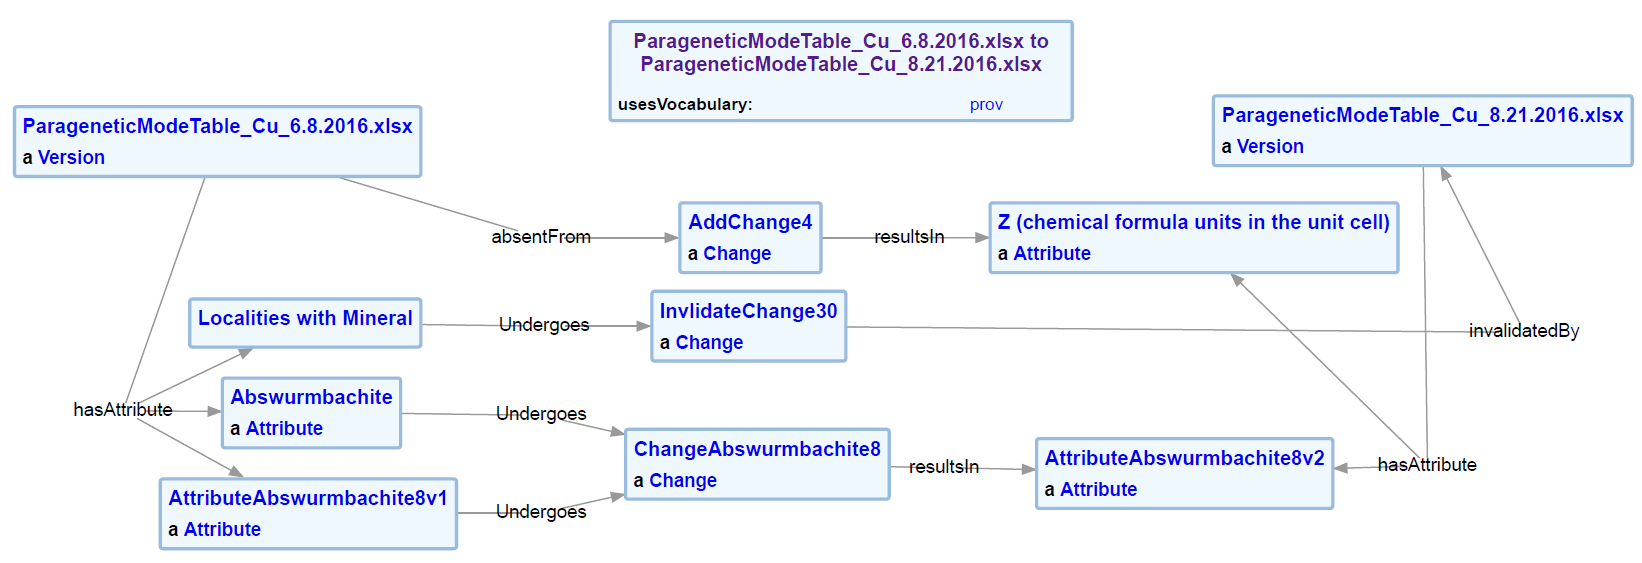
\includegraphics[scale=0.5]{figures/VersioningGraph2.png}%
	\end{adjustbox}
	\label{CopperGraphVerGraph}
\end{figure}

\subsection{Graphs with Multiple Versions}\label{sec:multiver}

Figures \ref{NobleGraph1} and \ref{CopperGraphVerGraph} depict a comparison between only two versions, but a project can contain more than two objects.
Case in point, a third version of the Noble Gas data set was released on July 11, 2017.
Figure \ref{NobleGraph2} shows a subgraph that contains changes from all three versions of the Noble Gas data set.
From the first to second version of the data, EGY001 becomes introduced as an attribute into the data set.
This entry then undergoes a modification change in columns 29, 31, and 43 when comparing versions two and three.
Entry TUR030 goes through a modification change in column 11 from version one to version two.
The entire row, however, becomes invalidated in version three.

\begin{figure}
	\centering
	\begin{adjustbox}{addcode={\begin{minipage}{\width}}{
					\caption{Versioning Graph representing the linked data graph with selected entries of additions, invalidations, and modifications after the publication of the third version. 
			}\end{minipage}},rotate=90,center}
		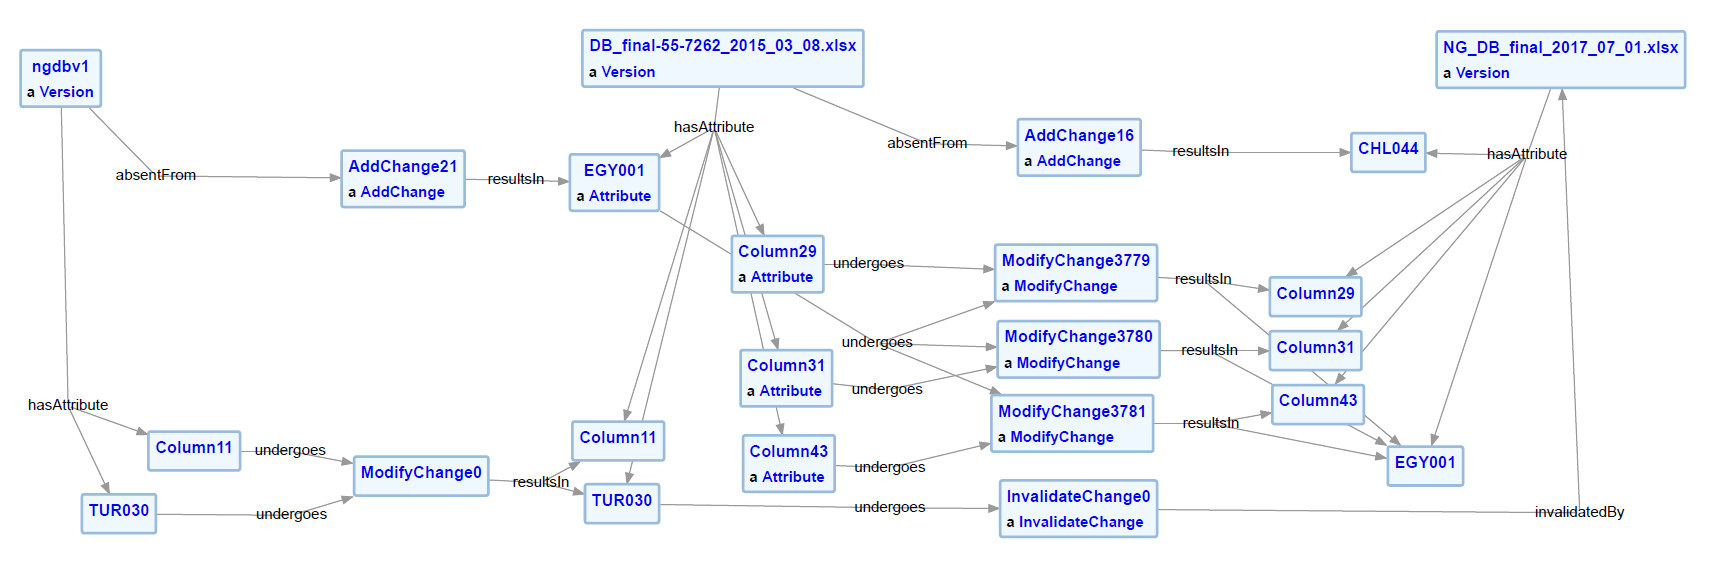
\includegraphics[scale=0.5]{figures/NobleVersion2.png}%
	\end{adjustbox}
	\label{NobleGraph2}
\end{figure}

Notice the difference in how Figure \ref{NobleGraph1} and Figure \ref{NobleGraph2} refer to columns.
Figure \ref{NobleGraph1} used linked data extracted from a change log employing RDFa, forcing the row identifier and the column identifier into the same concept.
The way nesting works in RDFa means that ChangeCAM00111 cannot back reference multiple concepts in a single statement, therefore AttributeCAM00111v2 was used to imply CAM001.
Figure \ref{NobleGraph2} used linked data extracted from a JSON-LD encoded change log.
Since the log can use explicit statements, the column identifier refers to the entire column and can be used to identifier changes in the same column across multiple rows.

\section{GCMD}

\subsection{GCMD Versioning Graph}

The Global Change Master Directory establishes the context that each \textbf{manifestation} of their keyword list are related versions.
Since the unique identifier for each keyword remains the same across versions, they can be used to align a mapping across versions.
\textbf{Additions} and \textbf{invalidations} are detected by checking an identifier's presence within both versions.
A \textbf{modification} occurs when a keyword's \textit{skos:Broader} property differs between adjacent versions.
A difference indicates that the word has been moved to a different place within the taxonomy since identifiers do not change across versions and a keyword only has one parent concept.
Changes over consecutive versions can be collected into a single graph using the method in Section \ref{sec:multiver} to chain together versioning graphs.
A change log was generated for each pair of consecutive versions in GCMD Keywords and embedded with JSON-LD.
Versioning graphs for each adjacent version was created by extracting JSON-LD from the corresponding change log, and entering the triples into a Fuseki triple store.

\subsection{Connecting Change Counts to Identifiers}

The \textbf{add}, \textbf{invalidate}, and \textbf{modify} counts for each transition are presented in Figure \ref{GCMDC1}.
The query used to extract the counts is found in Listing \ref{gcmd_list}.
Notice the sharp spike in adds and invalidates when transitioning from version 8.4.1 to 8.5.
The version identifiers indicate that at most a minor or technical change has occurred, but the counts of \textbf{addition} and \textbf{invalidation} changes in this transition is more than triple the counts in either of the previous \textbf{major} transitions.
Not only should a small transition not produce changes of this quantity, but the data set's size is on the order magnitude of the recorded \textbf{invalidates}.
In addition, no \textbf{modifications} are revealed, and even the root node "Science Keywords" has been invalidated.
Further investigation of the root word reveals that the name space for the keywords has changed from HTTP to HTTPS.
To provide context, NASA mandated a transition to secure protocols, and the group changed the name space to ensure the URIs remained resolvable.
Since the identifiers are unique, the new name space means they no longer refer to the same object after the protocol change.
Because the keyword identifiers no longer match, the mapping approach results in the total invalidation of keywords from 8.4.1 and the addition of keywords from 8.5.
The dot decimal identifier for the transition from version 8.4.1 to 8.5 does not match the number of changes in the versioning graph.

\begin{figure}[b]
	\centering
	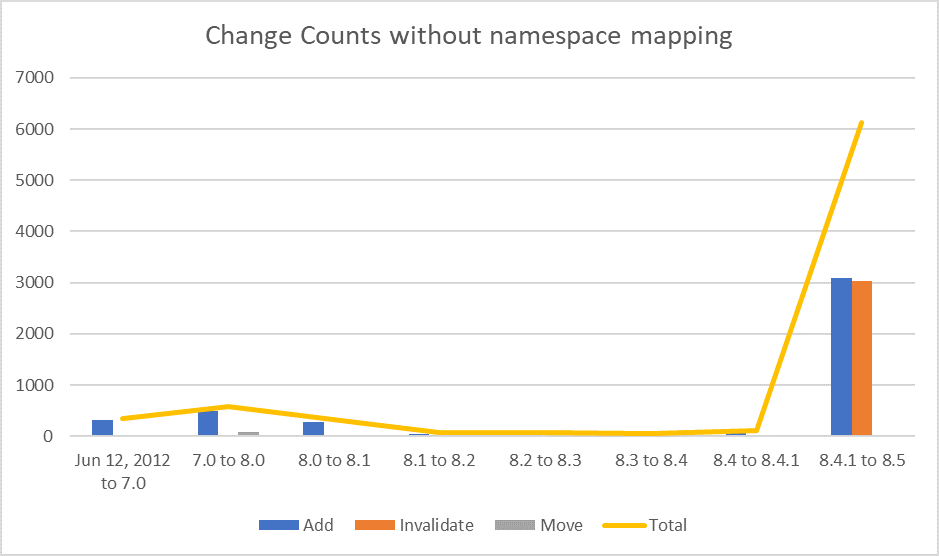
\includegraphics[scale=1]{figures/GCMDChart1.png}
	\caption{Add, Invalidate, and Modify counts in Version 8.5.  The counts show change magnitudes and indicate that major and minor changes differ by orders of magnitude.}
	\label{GCMDC1}
\end{figure}

%\hfill \break
\begin{lstlisting}[language=SPARQL, caption=This query compiles the counts for each subclass of Change in a GCMD versioning graph,label=gcmd_list]
PREFIX vo:<http://orion.tw.rpi.edu/~blee/VersionOntology.owl>
PREFIX rdfs:<http://www.w3.org/2000/01/rdf-schema#>

SELECT ?p (COUNT (DISTINCT ?s) as ?count)
{
?s a ?p .
?p rdfs:subClassOf vo:Change .
} GROUP BY ?p
\end{lstlisting}

Changing the mapping method to account for the new namespace provides a pathway to compare the perceived change by the producer as evidenced by the version identifier with the amount of change in the versioning graph.
To do this, the mapping treats identifiers with HTTP and HTTPS the same. 
Differences in change magnitudes become much clearer after controlling for the altered name space in Figure \ref{GCMDC2}.
All revisions are dominated by \textbf{additions}, but major version changes have counts around 300 to 500 while minor revisions are an order of magnitude smaller.
The transition from version 8.4.1 to 8.5 also seems to follow this trend.
The \textbf{additions} in ``8.4 to 8.4.1" in Figure \ref{GCMDC2} numbers almost a hundred, providing evidence that the trend of decreasing order of magnitudes may now continue as the granularity of the version identifier increases.

\begin{figure}%[b]
	\centering
	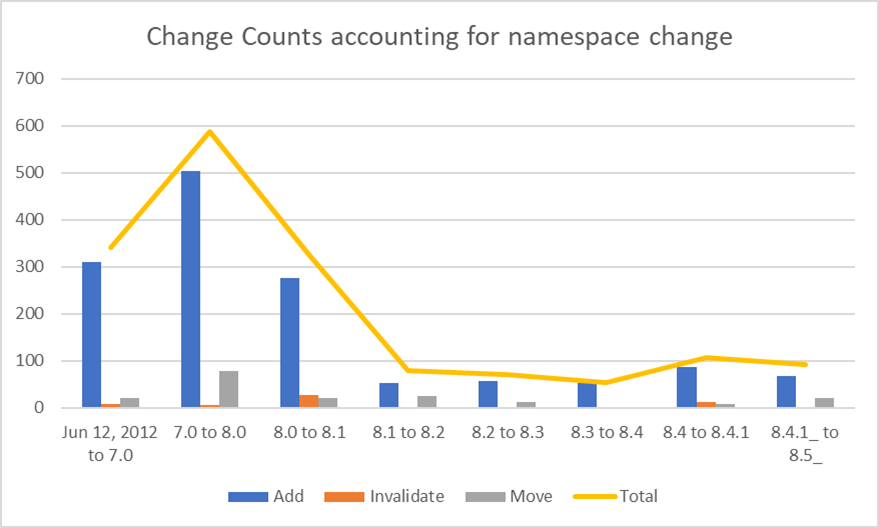
\includegraphics[scale=1]{figures/GCMDChart2.png}
	\caption{Add, Invalidate, and Modify counts ignoring the namespace changes in Version 8.5.  The counts show change magnitudes appropriate for the identifier.}
	\label{GCMDC2}
\end{figure}

\section{MBVL}


\subsection{Variant Versioning Graph}

The experiment conducts activity over two phases in this procedure.
The first phase takes sequences from the original known population and feeds the sequences though a particular algorithm/taxonomy combination to produce a candidate classification.
Since the classifications for the known population sequences is unavailable, there is not sufficient context to perform a valid comparison with the candidate classifications.
The second phase compares the performances of each candidate classification of a algorithm/taxonomy pair.
The use of \textbf{add}, \textbf{invalidate}, and \textbf{modify} varies slightly in this application since all the results use the same sequences.
A versioning graph utilizing just the sequence identifiers would only result in \textbf{modify} changes when taxonomic ranks differ since the sequence identifier exists in both data sets.
The mapping instead uses the sequence identifiers to align comparisons and then the taxonomic rank classification to determine the kind of change.
If the right-hand result specifies more taxonomic ranks, the relationship is an \textbf{addition}.
If the left-hand result is more specific, then the relationship is classified as an \textbf{invalidation}.
If both results have the same precision but the name differs, then the link is a \textbf{modification}.
Otherwise, no change is detected.

Figure \ref{mbvl_chart} shows the changes detected when varying either the taxonomy or the classification algorithm.
\begin{figure}
	\centering
	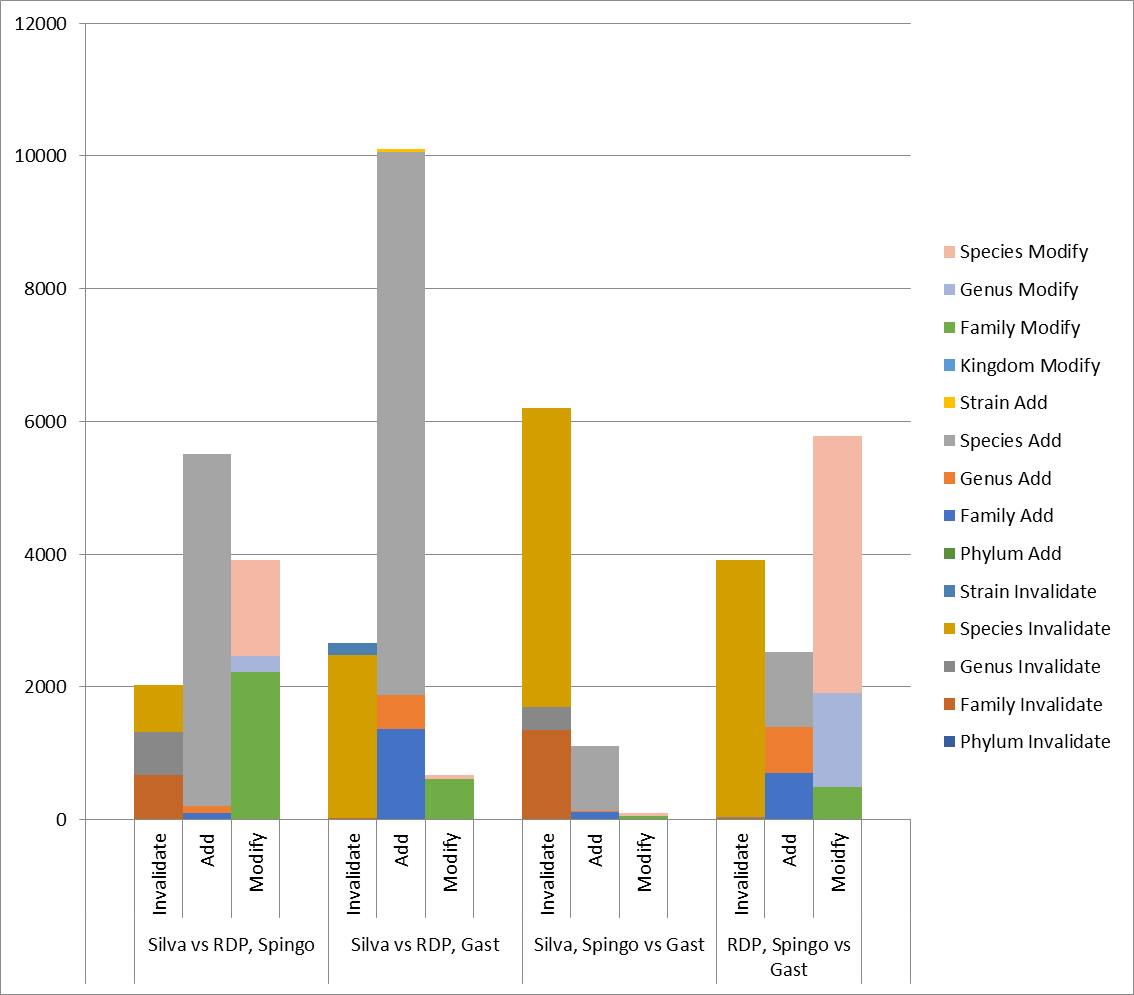
\includegraphics[scale=0.80]{figures/mbvl_chart.png}
	\caption{Compiled counts of \textbf{adds}, \textbf{invalidates}, and \textbf{modifies} grouped by taxonomic rank across algorithm and taxonomy combinations.}
	\label{mbvl_chart}
\end{figure}
No comparison was conducted with different taxonomy and classifier since that would introduce too many sources of variability to differing results in a classification.
Each bar indicates the total number of differences between sequences for a specific kind of change.
The bars are further broken down by the taxonomic rank at which the difference occurred.
For example, in ``Silva vs RDP, Gast", a notable number of classifications differed at the species rank.
The graph also indicates that using the RDP taxonomy often produces more precise classifications since both ``Silva vs RDP, Spingo" and ``Silva vs RDP, Gast" feature a larger number of \textbf{additions} than any other change.
The classifier comparisons feature a high number of \textbf{invalidations}; however, ``RDP, Spingo vs Gast" also displays a higher number of \textbf{modifications} than \textbf{invalidations}.


\section{Summary}

The results in this chapter implements the versioning model and demonstrates the process and challenges experienced in this endeavor.
The entries in a data set is separated into groups of additions, invalidations, modifications, and unmodified by their attributes.
These groups organizes the data into a form to publish into change logs which are much less restricted when encoded using JSON-LD rather than RDFa.
The resulting logs end up very large and sometimes do not load in a browser.
The versioning graphs for GCMD Keywords seem to indicate that there may be a relationship between change counts and version identifiers.
Finally, the MBVL data set demonstrates a case where versioning graphs can be used to compare the performance of different taxonomy/algorithm pairings.